
\chapter{Meteostanice}

    Meteostanice je zařízení, které pomocí řady čidel a senzorů sleduje a analyzuje počasí~\cite{JakVybratCHytrouMeteostanici}. V České republice existuje síť automatizovaných meteostanic, kterou spravuje Český hydrometeorologický úřad. Z naměřených meteorologických dat se tvoří numerické modely, díky nimž je možné předpovídat počasí~\cite{ChytraPetr}. Jednotlivé stanice měří především teplotu vzduchu, vlhkost vzduchu, atmosférický tlak, rychlost a směr větru, úhrn srážek a další. Pro možnost sjednocení a porovnání hodnot mezi různými meteostanicemi existuje dohoda například pro umístění měřících přístrojů. Čidla pro měření teploty, vlhkosti a atmosférického tlaku jsou umístěna v takzvaném radiačním krytu, ve kterém jsou chráněna před slunečním svitem~\cite{ChytraPetr}. Pro správné měření však musí být skrz kryt umožněno proudění vzduchu. Teplota vzduchu se většinou měří ve výšce 2 metry nad zemí s rozlišením 0,1 °C. Naměřený atmosférický tlak se kvůli porovnání na více místech přepočítává na tlak v úrovni hladiny moře, jelikož na stejném místě se atmosférický tlak mění v závislosti na nadmořské výšce~\cite{ChytraPetr}.
    
    Kromě těchto profesionálních meteostanic však existuje nespočet dalších, ať už amatérských, nebo komerčně vyráběných zařízení pro domácí použití fungujících na podobném principu. Takové meteostanice nabízí například výrobci: Sencor, GARNI, EMOS, ThermoPro, Hyundai a další~\cite{Meteostanice}. Pro porovnání jsem vybral následující: 

    \section{Hyundai WS 2303 černá}
        Meteostanice nabízí animovanou předpověď počasí na nejbližší hodiny, měří venkovní i vnitřní teplotu a venkovní vlhkost. Uchovává v paměti maximální a minimální hodnoty vnitřních i venkovních senzorů. Předpověď i aktuální data, fáze Měsíce a přesný čas řízený rádiovým signálem se zobrazují na barevném LCD displeji na vnitřní jednotce, kterou můžete vidět na obrázku~\ref{hyundaiWS}. Naměřená venkovní data se do vnitřní jednotky přenáší rádiovým signálem (433 MHz). Napájení vnitřní jednotky je řešeno adaptérem ze sítě. Venkovní jednotka je napájena dvěma 1,5V AAA bateriemi~\cite{HyundayWS2303}. Cena je 999 Kč
        
        \begin{figure}[htb]
        \resizebox{8cm}{!}{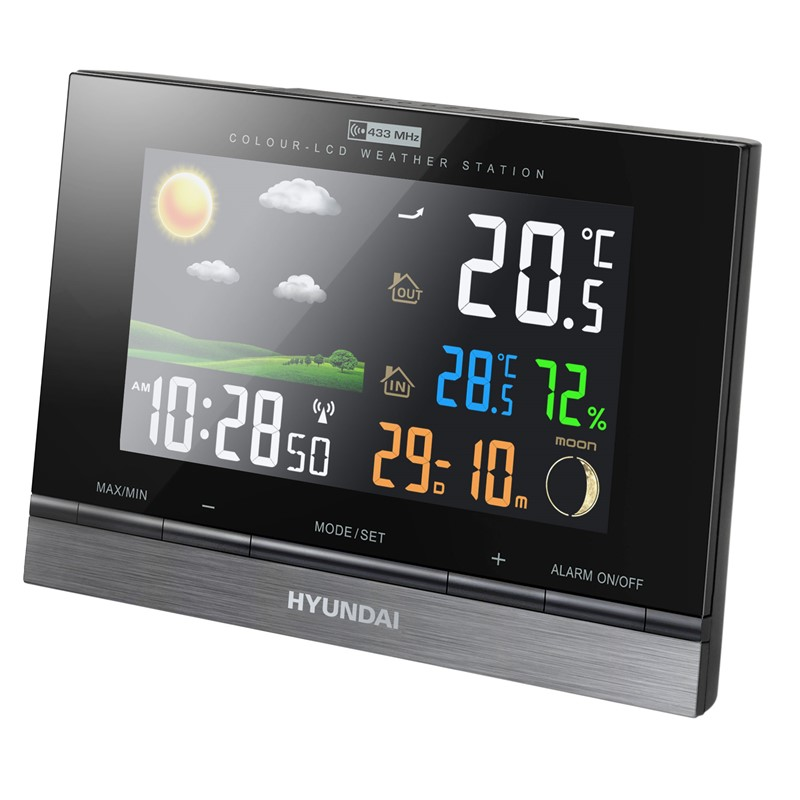
\includegraphics{LaTeX sablona IB/obrazky/hyundai.jpg}}
        \caption{meteostanice Hyundai WS 2303~\cite{WS2303Obrazek}}
        \label{hyundaiWS}
        \end{figure}

    \section{Sencor SWS 12500 WiFi}
        Základem meteostanice je hlavní jednotka, která nabízí přehledná data na displeji a uživatelská tlačítka (obr.~\ref{sencorWS}). K hlavní jednotce lze připojit až 7~bezdrátových vnitřních čidel, měřících teplotu a vlhkost a jednu venkovní jednotku 7v1, která měří teplotu, vlhkost, tlak, rychlost a směr větru, intenzitu světla, intenzitu UV záření a srážky. Naměřené údaje se prostřednictvím WiFi posílají do řídicí jednotky, která je zobrazuje a vytváří předpověď počasí na 12 až 24 hodin dopředu~\cite{SWS12500WIFI}.
        
        Veškerá data jsou dostupná online v mobilní aplikaci, meteostanice podporuje veřejné platformy Weathercloud, Weather Underground a Počasí Meteo, do kterých jsou zapojeni uživatelé z celého světa a přispívají daty ze svých stanic. Cena je 4799 Kč~\cite{SWS12500WIFI}.
        
        \begin{figure}[htb]
        \resizebox{8cm}{!}{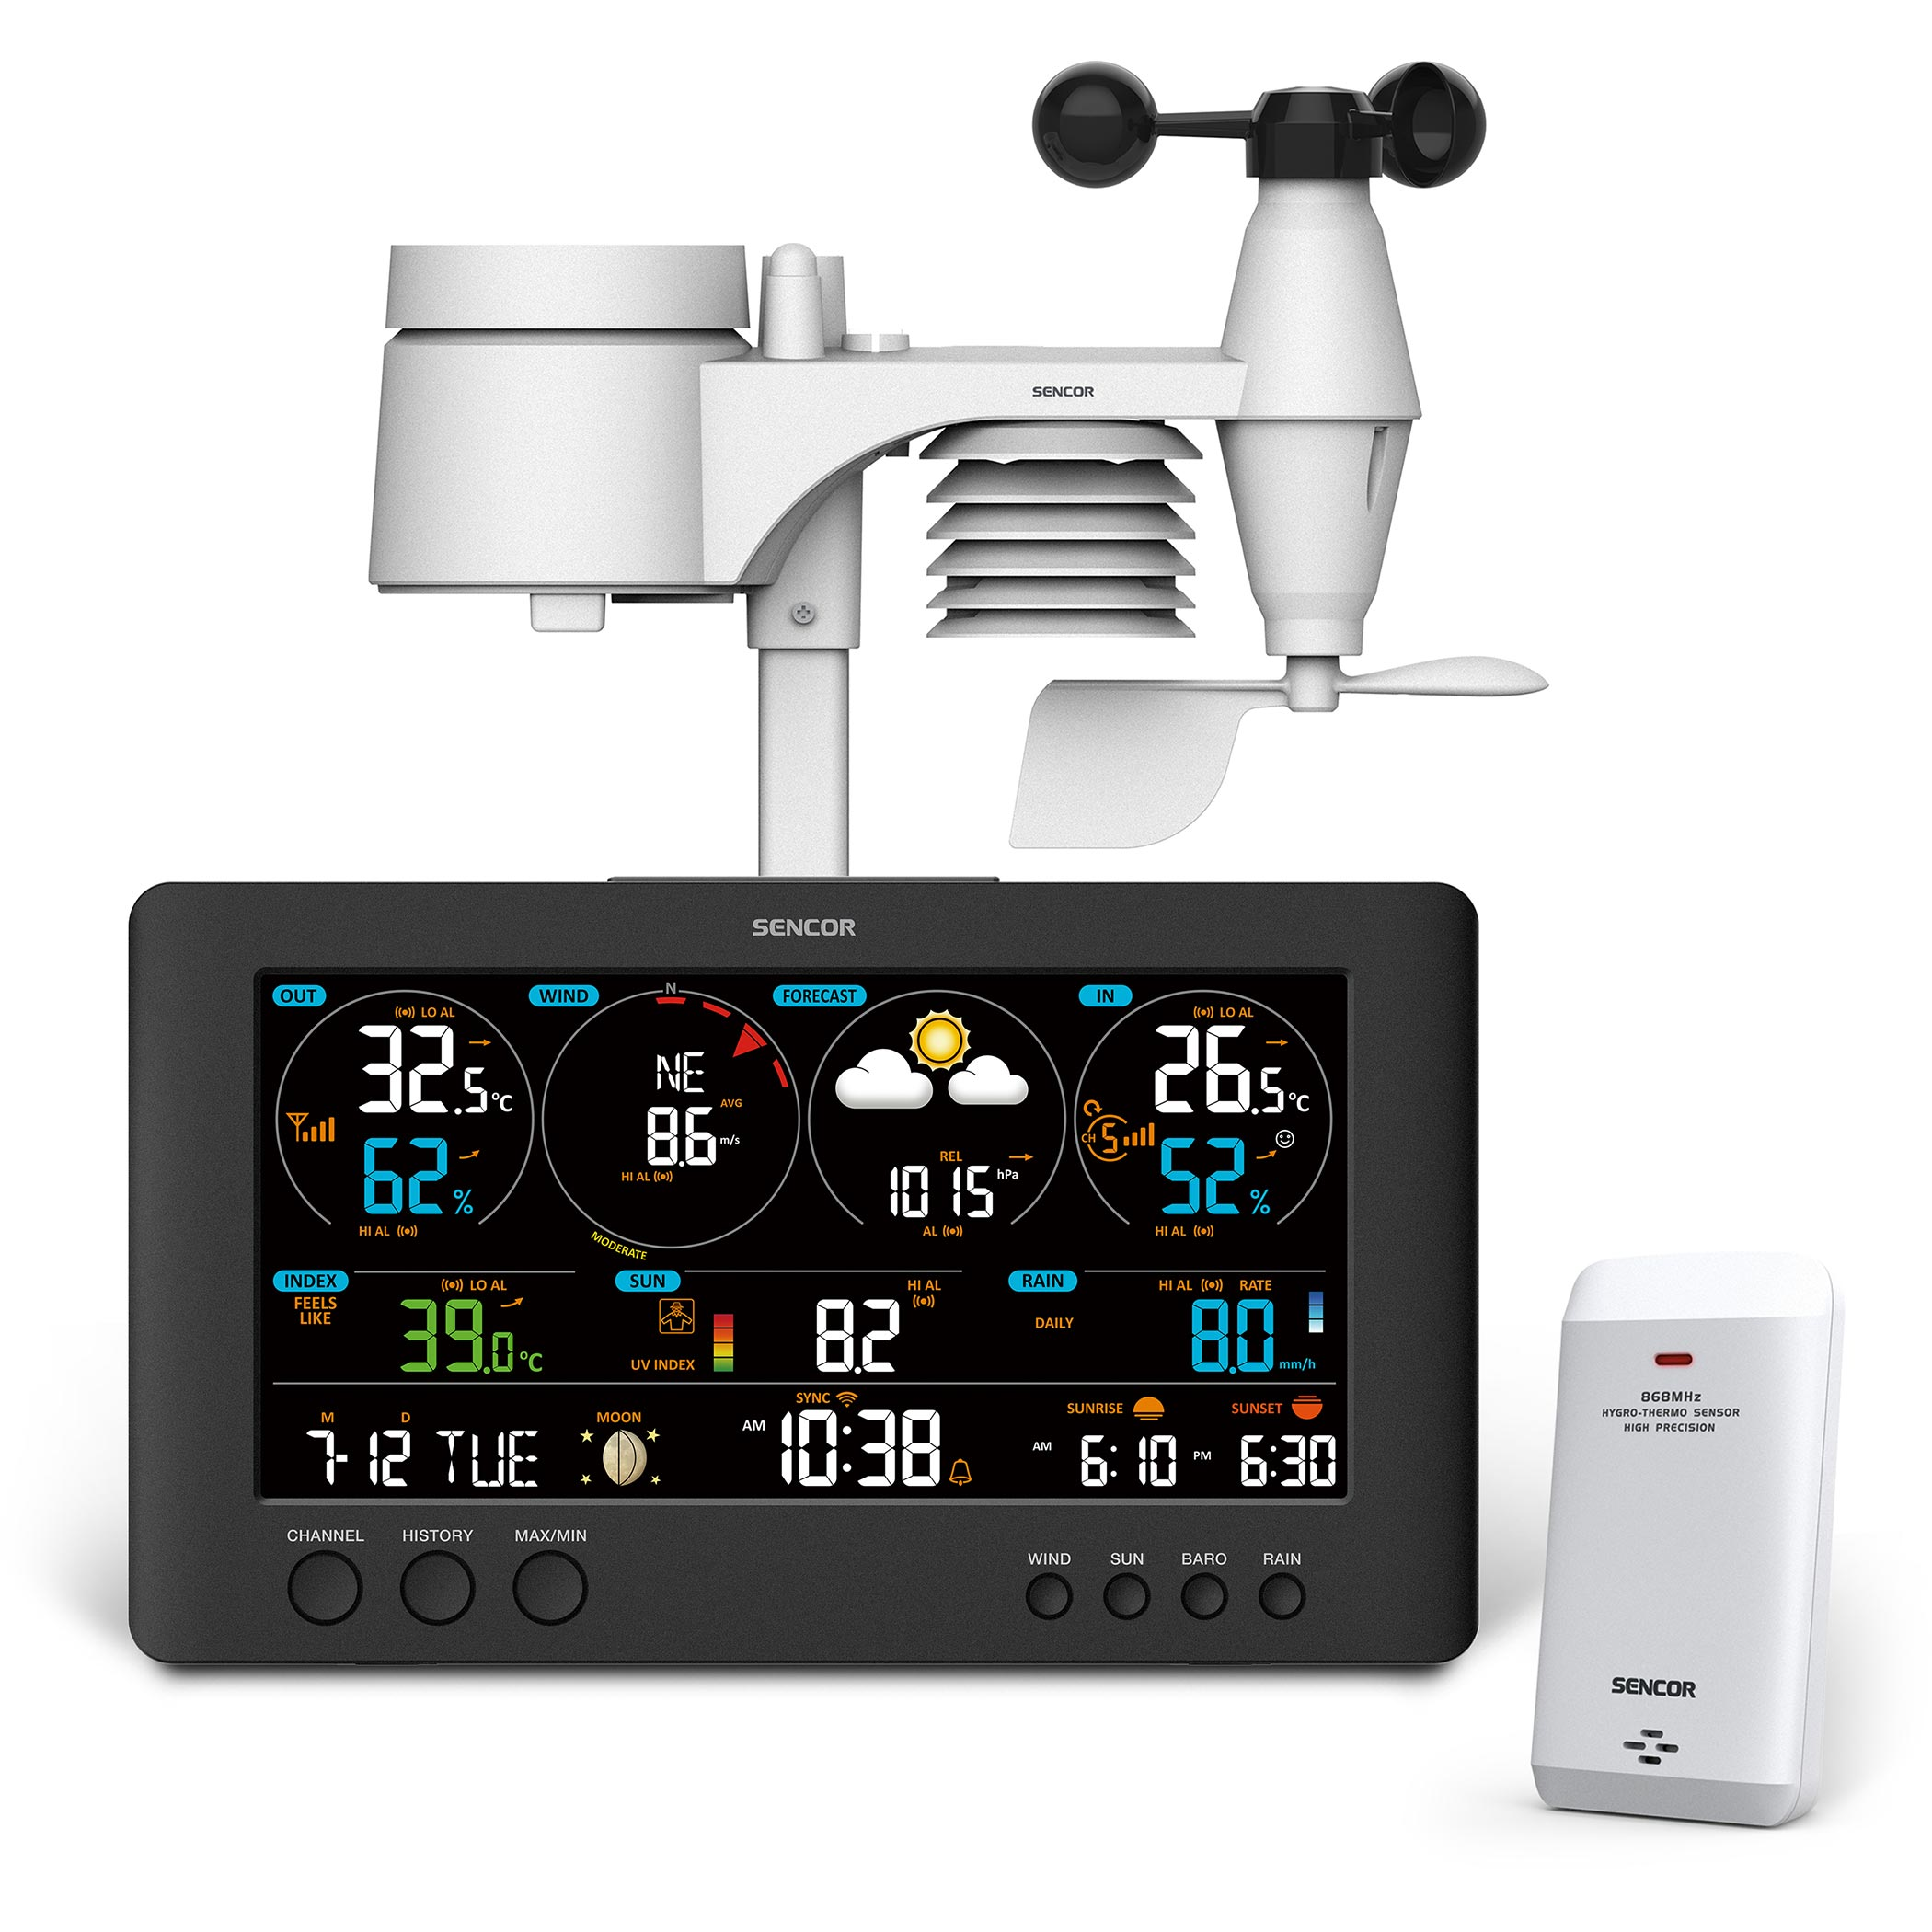
\includegraphics{LaTeX sablona IB/obrazky/sencor.jpg}}
        \caption{meteostanice Sencor SWS 12500 WiFi~\cite{SWS12500Obrazek}}
        \label{sencorWS}
        \end{figure}